%=========================================================================
% sec-accelerator
%=========================================================================

\section{Accelerator Subsystem Functional RTL Verification Strategy}

\fixme{cut-and-paste from Rajesh/Mani -- I still need to take a pass}

Untimed blocks consist of functional or imperative code blocks captured
as functions, processes and modules. While functions/procedures represent
well-defined algorithmic behaviors, processes represent non-terminating
behaviors. Modules are characterized by structural interfaces that
provide the basic unit of composition for the SOC design (see Figure
below). Algorithmic design proceeds by a ``bottom-up'' development of the
functional specification that is refined into an implementation in a
programming language of choice. Architectural design proceeds by a
``top-down'' decomposition of functional blocks that is refined into an
implementation. The two process run simultaneously providing ample
opportunities for architecture-algorithm co-design by means of
``compositional glue'' that enables simultaneous execution of
heterogeneous functional blocks.

Within the context of the CRAFT/CERTUS project, we have applied this
co-design methodology in the design of a neural network accelerator that
is composed with a predesigned RISC-V Rocketcore. There are two parts to
a neural network design: determination of the matrix weights through an
extensive ``training phase'' that is done offline. A trained network is
implemented and used for a variety of ``recognition'' tasks (as one of
the inferences that can be derived using a neural network.) We start with
algorithmic description of a convolutional neural network (CNN)
consisting of layers of processing. The CNN is typically described by
means of data-flow graphs by algorithm designers and implemented using
high-level libraries such as Theano Deep Learning Framework.

The starting point of algorithmic design in CERTUS project is a manually
entered description of CNN in Python using Theano. As a part of our SOC
strategy, CERTUS uses a novel binarized CNN or BNN that goes far beyond
preliminary BNN implementations in the literature in that it binarizes
both the weights as well as the gradient calculations. As a part of
algorithmic design, the team implemented a BNN that provides the right
balance of accuracy versus model size compared to a conventional CNN. We
also explore methods to speed up computation of CNN via spectral
decomposition method that is described elsewhere. The process of
algorithmic design is done using Theano and tested using MNIST and CFAR10
benchmarks images. This also includes the process of binarization,
neither of these are subject to CERTUS SOC validation methodology since
they are part of the algorithmic design process. The result of
algorithmic design process is creation of a ``golden reference model''
against which all subsequent validations take place (see Figure below).

In the BNN acceleration algorithm implemented in CERTUS, we binarize both
weights and activations of the network. This reduces the size of
parameters and changes the arithmetic operations into bitwise operations
thus accelerating the inference algorithm. The implementation of BNN
includes reading the Python-trained BNN model parameters to the BNN
network and classification of the CIFAR10 image dataset. The network is
composed to six convolutional layers with 3x3 filters, three 2x2 padding
layers and three fully-connected layers.

We compared the performance of CERTUS BNN accelerator with the original
floating-point Convolutional Neural Network, and use testing dataset of
CIFAR10 to get the image classification error-rate. The BNN model can
achieve about 11.4\% error-rate. This result is close to the
state-of-the-art CIFAR10 classification result, while having a higher
computation speed and smaller memory requirement.

%=========================================================================
% fig-verification-hls
%=========================================================================

\begin{figure}
  \centering
  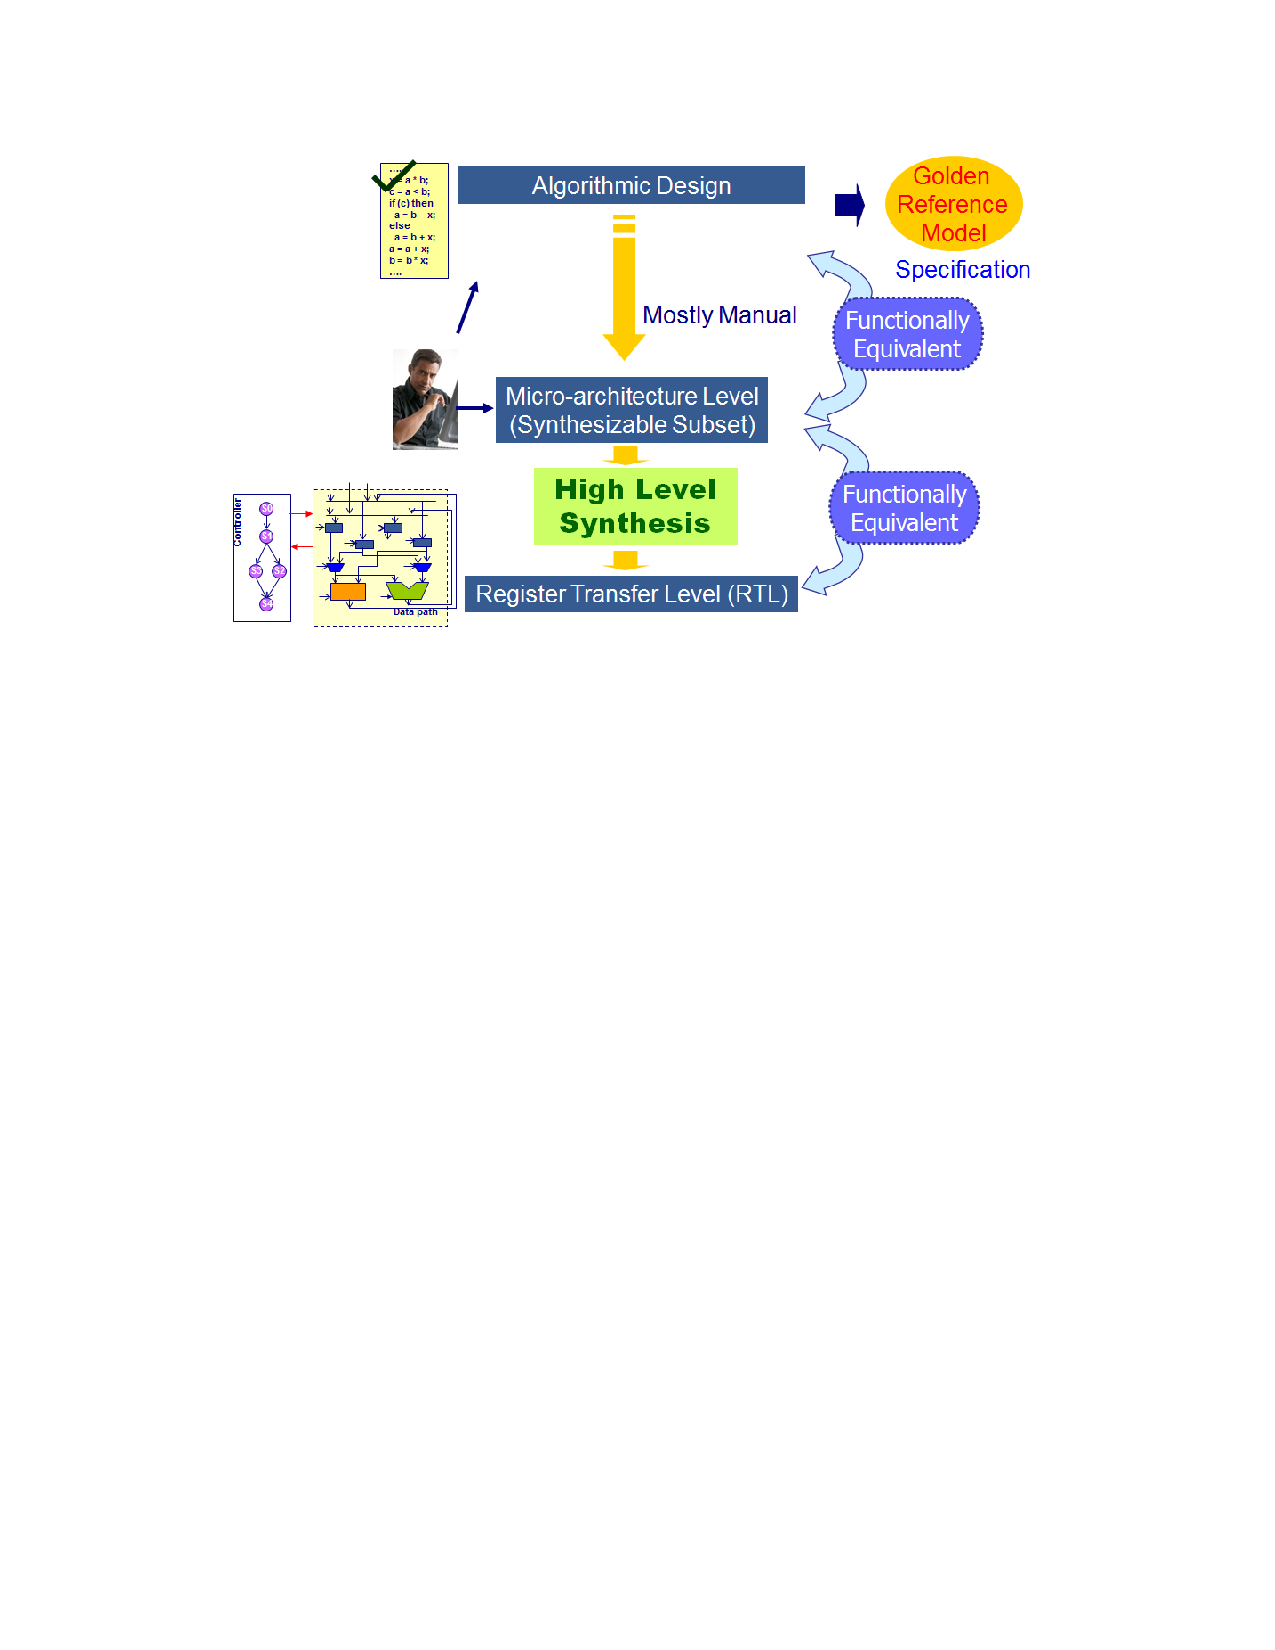
\includegraphics[width=0.7\tw]{verification-hls.pdf}
  \caption{\BF{Verification for High-Level Synthesis}}
  \label{fig-verification-hls}
\end{figure}



\BF{Architectural Design and Implementation}

The entire process of binarization of the CNN algorithm is conducted in
Python. Once we have converged on the quality of binarized CNN results,
the SOC accelerator design process starts. We start with a reference
model in Python/Theano where design refinement into implementation
compares results of layer-by-layer computations on image benchmarks
against the reference implementation. There is no approximation in the
feedforward stage and hence this comparison can be made to exact
numerical values. Indeed, the process of binarization in CNN actually
assists in validation since the layer computation results can now be
compared to be bitwise identical to the reference implementation.

As a part of algorithm design, the BNN network models were trained in
Theano in Python. We trained various models for different settings:
original BNN, reduced BNN, BNN without bias, and BNN with non-zero
padding values. These various algorithmic choices were analyzed for
performance and model size. The algorithm design group handed off
reference Python code and all trained models to the SOC accelerator
design team for implementation in hardware.

For BNN verification in algorithm level, we compared the output values of
C program with Python program for each layer in the BNN network. These
have the same values throughout the network and their final output are
also identical. So the BNN in C program is in accordance with the
theoretical BNN network we designed and also the BNN model we implemented
in Python.

For Hardware implementation verification, we provided the C and Python
programs and model parameters, along with the expected output of CIFAR10
dataset to accelerator architectural design group at Cornell. The output
of the Python program provides the golden reference model that is used in
validating the architectural implementation of BNN hardware.

\fixme{cut-and-paste from Zhiru -- I still need to take a pass}

The design of the BNN accelerator employs an incremental approach for
bringing the algorithm specified in high-level program to low-level
synthesized RTL. Likewise, our verification methodology features tests at
each stage of the design flow to ensure that errors are not propagated in
between different stages of the model. Based on this principle, we first
verify that our C++ model implements the intended algorithm and executes
in consistency with published Python implementation. We then verify that
the generated RTL from C++ functions as intended by the C++ model. At
last, we verify the correctness of our SystemC model and its generated
RTL using the same set of tests from C++.

While we utilize standard software testing practices for verifying the
correctness of the Python, C++, and SystemC specifications, we leverage
co-simulation infrastructures in HLS tools to verify the correctness of
the generated RTLs. Our verification flow benefits from advances in
co-simulation which allows direct reuse of the original software
testbenches to drive RTL simulation on the generated accelerator.
Co-simulation significantly alleviates verification effort by avoiding
the need for timing-consuming manual creation of RTL testbench.

\BF{Verifying C++ model against the algorithm}

The simplest test ensures that the C++ model performs 3D convolution and
binarization correctly. This done by a testbench called test-random,
which verifies the C++ model on a set of randomly generated feature maps
and conv filters. The model reads in the random data and produces a
single output binary feature map, which is compared against the output of
a golden reference model written in a simple mathematically manner.

The random test is the smallest available test and its number of input
images can be easily scaled as they are randomly generated. However, it
only tests a single output image. Furthermore, it does not test the input
conv layer, the dense layers, or max pooling.

\BF{Verifying C++ model against Python}

Further verification compares the BNN C++ model against the Python code
on a layer-by-layer basis. Intermediate feature maps from the Python
program were first dumped to disk. The testbench test-layer then verifies
any one layer by sending in the dumped input feature maps and comparing
the output with the dumped output feature maps. Note that due to hardware
model optimizations (fixed-point, etc) there will be some discrepancy in
the results, but the expected rate of incorrect bits on a single layer is
less than 2\%.

The layer test is extremely useful as there are three functions/modules
in the BNN corresponding to the three layer types: input conv, binary
conv, and dense. This test verifies each of these functions in isolation.

The last and most comprehensive test is test-full, which tests the entire
BNN by sending in CIFAR-10 test images and checking the output class
labels as generated by the Python code. The test can be scaled between 1
and 10000 test images. Again, the hardware model optimizations mean that
the accuracy over 10000 images may not match that of the Python
reference. However, the accuracy difference is negligible (less than
0.5\%).

\BF{Verifying C++ HLS-generated RTL}

The HLS-generated RTL is tested in two ways. The first is through Vivado
HLS' co-simulation feature. Because co-sim is quite slow, only
test-random was executed.

The second method is to generate the FPGA bitstream and run test-full
with all 10000 images on a real FPGA board. This tests the accuracy of
the BNN in real hardware, and ensures the accuracy matches that of the
C++ model. Board testing also enables measurement of the execution time
and examination of possible latency bugs.

\BF{Verifying SystemC model}

Because our SystemC is ported line-by-line from our C++ model except for
SystemC-specific constructs and interfaces, we can conveniently reuse
many of the testbenches developed for verifying the C++ model. As a
result, we were able to perform all three available tests - test\_random,
test\_layer, and test-full on our SystemC design.

Similar to the C++ testing flow, we first performed SystemC (behavioral)
simulation to verify the correctness of the SystemC functional
specifications. Because this is a software simulation, we were able to
run all three available tests, including test-full with all 10 images.
Once the SystemC model has been verified behaviorally, we then perform
SystemC-RTL co-simulation to verify the correctness of the generated RTL.
We were also able to run all three available tests. However, given the
speed of RTL simulation, we run test-full on only 4 images.

\BF{Verifying correctness of SystemC synthesis}

A major roadblock on our design flow stemmed from bugs inherent in the
SystemC-to-RTL synthesis process. We were experiencing mismatches between
results from behavioral simulation and RTL simulation.

Our strategy relied on using SystemC print statements that can be
synthesized into SystemVerilog prints so we can conveniently compare the
behavioral simulation printouts to the RTL simulation printouts to
localize mismatches. Once we localized the mismatches, we created unit
test cases that specifically target these mismatches. If needed, we
examined the waveforms for these unit test cases to identify errors that
were otherwise not obvious. In general, memory bugs are easier to detect
with waveforms because our SystemC synthesis preserves the names for
memory elements.

